\section{Original Simulator}
\label{sec:simulator_aloha}

The simulator is event driven and implemented in plain Python.
Events are stored in a priority queue, where the priority is given by the timestamp of the event.
The simulator loops over the events queue, until the wanted simulation time is reached.
At each iteration, the first event is extracted from the queue and precessed.
Each step can change the internal state of the simulator, schedule new events and generate logs, which are collected in a log file.
The produced logs are used to compute metrics that can be used to evaluate the overall performances of the simulated system.

\begin{figure}[h]
	\centering
	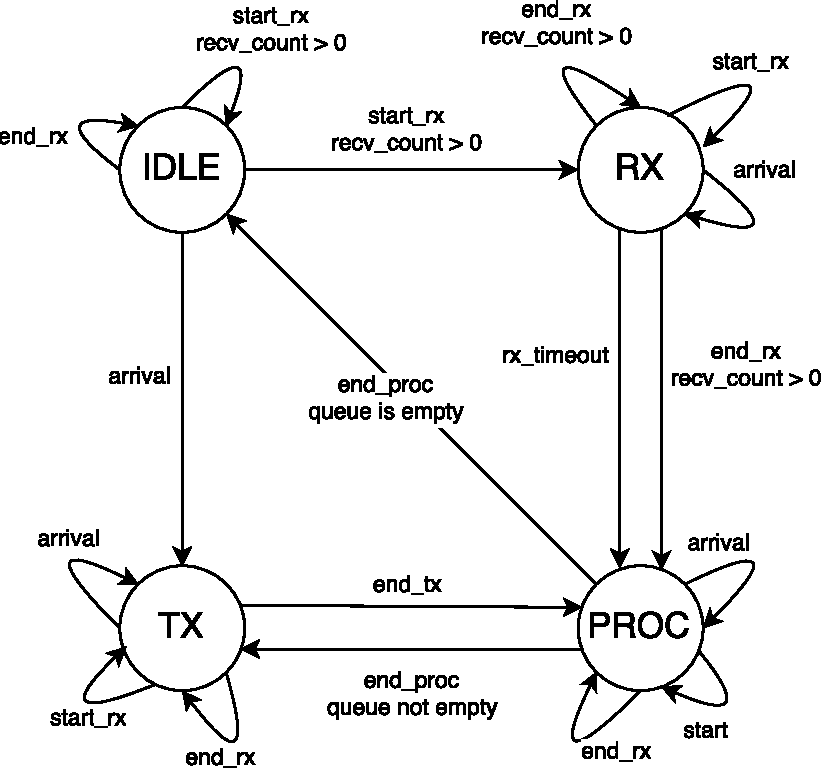
\includegraphics[width=0.88\columnwidth]{figures/states/aloha}
	\caption{State machine for a single station for Aloha. Stations can be in $4$ different states, represented by the circles. Arrows indicate the transitions from one state to the other on a given event.}
	\label{fig:aloha_states}
\end{figure}

\cref{fig:aloha_states} shows the possible states of a station:

\begin{itemize}
    \item \textbf{IDLE} - the station is not doing anything,
    \item \textbf{RX} - the station is receiving a packet,
    \item \textbf{TX} - the station is transmitting a packet,
    \item \textbf{PROC} - the station is processing the last packet.
\end{itemize}

The behaviour of a station is determined by its state, the packets that are currently being received (\texttt{recv\_count}) and the length of its queue.
If multiple packets arrive at the same time, they collide and the simulator marks them as corrupted.

Each packet need some time to be propagated through the channel and some other time to be received from a station, depending on the packet size.
The size of the packets and their interarrival time are computed using random values taken from some distribution.
The distributions and their parameters can be configured in the configuration file.

The events used in the simulator are:

\begin{itemize}
    \item \textbf{arrival} - a new packet to transmit arrives to the station,
    \item \textbf{start\_rx} - the station starts to receive a packet,
    \item \textbf{end\_rx} - the station finishes to receive a packet,
    \item \textbf{end\_tx} - the station finished to transmit a packet,
    \item \textbf{end\_proc} - the station finished to process a packet,
    \item \textbf{rx\_timeout} - the maximum time allowed to receive the packet is over, the packet is probably corrupted and must be discarded.
\end{itemize}

The simulator schedules the first packet arrival on each node.
Packets are transmitted to all reachable nodes: the channel object compute the nodes to send the packet to and schedules, after some propagation time, an arrival on the receivers.
